% !TEX root = ../../thesis.tex

\cleartoleftpage
\includepdf{../media/chapter_illustration/papaver_rhoeas}



\chapter{The Poppy development} % (fold)


\section{Introduction} % (fold)

Research in humanoid robotics has been thriving in the recent years~\cite{hirai1998development} \cite{kaneko2008humanoid}, both due to theirs predicted relevance for personal and assistive robotics~\cite{tapus2007socially} \cite{oztop2005human}, and because of the scientific challenges raised by robotics with regards to cognition~\cite{asada2001cognitive}, natural communication~\cite{stiefelhagen2004natural} \cite{breazeal2002robots}, biped locomotion~\cite{yamaguchi1999development} \cite{chestnutt2005footstep} \cite{collins2005bipedal} and full-body physical interaction with the environment~\cite{ude2004programming}.

But like the LHC is an experimental platform allowing to explore quantum mechanics and the origin of our universe,  humanoid can act as simplified and controllable human simulator. Thus humanoid robots can be amazing tools to study human-being and eventually contribute in a better understanding of Human's behaviors and abilities~\cite{atkeson2000using} \cite{cheng2007cb} \cite{brooks1986achieving}.

A famous example of such humanoid uses was the Cog project~\cite{brooks1999cog} at the Humanoid Robotics Group of the Massachusetts Institute of Technology. This research project has two goals: an engineering goal of building a prototype general purpose flexible and dextrous autonomous robot and a scientific goal of understanding human cognition~\cite{brooks1994building}. In particular, this project concentrated on embodiment and interaction intelligence with four aspects of a novel methodology: developmental structure, physical embodiment, integration of multiple sensory and motor systems, and social interaction. For this purpose they build several robotic platform such a humanoid~\cite{brooks1999cog} (see \figurename~\ref{fig:brooks_and_cog}), and a very expressive multi-articulated head named Kismet~\cite{breazeal2003emotion} (see \figurename~\ref{fig:breazeal_kismet}).

% This project ended in 2003 and has bring great scientific contributions such as ... REF


\begin{figure}[t]
\centering
    \subfloat[][Rodney Brooks and the Cog humanoid]{\label{fig:brooks_and_cog}\includegraphics[height=5cm]{brooks_and_cog.jpg}}
    \hfil
    \subfloat[][Cynthia Breazeal with Kismet]{\label{fig:breazeal_kismet}\includegraphics[height=5cm]{breazeal_kismet.jpg}}
    \caption{The Cog project was about the use of computer and robotic technology to better understand and emulate human intelligence.}
    \label{fig:cog_project}
\end{figure}



The context of this PhD thesis is grounded on the same scientific motivations as the work of R.Brooks, R.Pfeifer, T.McGeer and initiative such as the Cog project i.e. exploring the role of morphology, cognition and embodiment intelligence in several aspects using real experimental robotic platforms.

The scientific approach of the Cog robots is oriented toward the exploration of embodiment in several aspects, from the low level mechatronics to head design for social interactions, but they were built 15 years ago and using classic manufacturing technique (see \figurename~\ref{fig:cog_project}) that made them expansive, complicated to be modified and especially difficult to diffuse in other laboratories.
We are now in 2014, the makers revolution is in progress~\cite{anderson} and novel technologies allows to rethink the way we design robotic platforms, especially humanoid.

In the previous chapter we presented a methodology to design robotic platform allowing both a free exploration of morphological variations and the diffusion in the research community. This method uses 3D printing to produce mechanical part, Arduino architecture for the electronic system and python-based API for the control.

We think such design methodology can contribute in building better experimental robots while it allows to make the modification of a robot morphology both easy and low cost, and by the use of open source diffusion, it permits the transfer and the reuse of scientific work in other laboratories.
Within this context we built a whole new humanoid robot called PoppyTM (see Fig.~\ref{fig:poppy_with_me}).

\begin{figure}[tb]
    \begin{center}
        \includegraphics[width=0.7\linewidth]{lapeyre_and_poppy.jpg}
    \end{center}
    \caption{Poppy}
    \label{fig:poppy_with_me}
\end{figure}

This humanoid robot is designed to easily and quickly conduct scientific experiments on sensorimotor learning, exploring morphological properties, and human-robot interaction. As an experimental robotic platform, Poppy is designed to be \textbf{affordable}, \textbf{lightweight}, \textbf{robust and safe}, \textbf{easy to use}, \textbf{highly-hackable} and \textbf{fast and easy to duplicate or modify} with the goal to be easily reproducible and used by other lab thanks to an open source distribution (hardware and software).

In this chapter,  we will describe our motivation, the design guidelines we have followed and the conception of Poppy.


\section{Creating a novel humanoid robot} % (fold)

\subsection{Motivations} % (fold)

In 2012, when we started this work, none of the existing humanoid platforms were suitable for exploring the role of morphology. There were two kind of platform. On one hand the commercial robots, rather easy to use and accessible but with a static and frozen morphology. On the other hand, prototype robots produced in labs to adresse specific experimentations, studying interesting morphologies but complicated to use and impossible to reproduce outside the lab.

In our lab, we had both kind of robot. We used Nao (see \figurename~\ref{fig:nao_platform}) to study human robot interaction (REF PIERRE cadeau). It was really convenient to be use by researchers those are not comfortable with get their hands dirty and do not really care about hardware issue while their are addressing more high-level research challenges. Yet such platform is limited as it is not possible to modify it if the robot is not adapted to our experiment. For example back at this time the Nao camera was not efficient, we have difficultly achieved 5 frames/seconds.
We had the necessary skills to hack Nao and change the camera but its hardware is not designed to be changed. Improving the vision performance could only be possible by the addition of an external camera on the Nao head which would ruin the user experience.

\begin{figure}[]
\centering
    \subfloat[][Nao]{\label{fig:nao_platform}\includegraphics[height=5cm]{nao_face.png}}
    \hfil
    \subfloat[][Darwin-Op]{\label{fig:darwin_platform}\includegraphics[height=5cm]{darwin_op_face.jpg}}
    \hfil
    \subfloat[][Acroban]{\label{fig:acroban_platform}\includegraphics[height=5cm]{acroban_wout_background.jpg}}
    \caption{None of the existing platform in 2012 was suitable to explore the role of morphology. Nao was impossible to modify. Darwin Op and Acroban used aluminium part really difficult and expensive to produce.}
    \label{fig:2012_Humanoids}
\end{figure}

We also used Acroban (see \figurename~\ref{fig:acroban_platform}) designed in our team by Olivier Ly~\cite{Ly2010}. It is a handcrafted humanoid platform created to explore morphological properties, especially compliance toward the achievement of dynamic locomotion and playful physical human robot interaction.
While it actually allows modification of its is morphology, its manufacture based on aluminum mechanical parts, Robotis Dynamixel motors, scotch, and rubber bands cobbled together therefore requires lot of effort to be changed. Especially the manufacture of aluminum parts require specific skills and tools.
Also its use was quite complicated and while several researchers could have been interested by Acroban to study human robot interaction and social acceptance, it was not possible to use it without getting our hands dirty.
Finally, the material and manufacture process make platform non-stationary, even if a lab manage to reproduce it, there is a high probability that the physical properties will not be the same. Therefore, the diffusion and the reproducibility of results are limited.


A last alternative would be the use of Darwin Op robot (see \figurename~\ref{fig:darwin_platform}) which is both open source and reproducible, yet as Acroban its hardware based on manufactured metal parts make its morphology difficult and expensive to be modified. Moreover to our knowledge, Darwin morphology has never be changed by the research community.

Thus one of the main goals was to achieve the design of a humanoid robot which can merge the advantages of both kind of robot, i.e. simple, accessible, reproducible and allowing to easily change and hack its morphology.

\subsection{A robot experiments-proof} % (fold)

Most researchers can attest of the difficulty and frustration raised by conducting robotic experimentation in the real world. We are daily challenged by bugs, technical issues, unpredicted events and side effects. While a bug in a software can be fixed, an error with a hardware platform can cause damages and postpone the results of an experiment by several weeks.

Therefore many robotic researchers avoid technical issues link with the real world experimentation by using simple model and physical simulation. But the real world is extremely more complex and rich than the virtual one.
Some high-level behavior experiments are conducted in simulator based on the hypothesis that the real world constraints are not relevant, yet it is really sure ?
Indeed, while the real world constitute a lot of constraints, it is also rich of complex physical effects (gravity, friction, inertia) which has to be took in and can be very useful if interacting with the agent.

As we saw in the related work (chapter~\ref{REF}), the emergence of complex behavior can appear thanks to the interaction between the real world and simple robotic system. We cannot program behavior while the behavior is the interaction resultant between the program and the real world. Thus we cannot design behavior without the ecological niche of the robot~\cite{Steels1991emergence}.

While using simulator can be helpful as a first step to design robot, it appears incomplete to show results on the role of morphology without real world experimentations.
Therefore, when ones want to study the role of morphology on the robot behavior, being able to explore it in the real world is of paramount importance.

Along our work on building cognitive and developmental learning algorithms, we had experienced these issues, especially while building and using Acroban~\cite{Ly2010} and during the Ergo robot experience (see section~\ref{REF}).

Therefore Poppy has been designed based on the experience background we have building and using robots acting in the real world.

\begin{description}
    \item[Robustness and Safety:] Heavy and long real-world experimentations imply a robot should be robust and safe. It should be able to sustain experiments and fall down without easily breaking. At the same time, one should ensure that physical interaction with the robot is safe for humans.
    \item [Precision, stationarity:]Experiments should be repeatable, implying that the robot properties should be stationary.
    \item [Breakable, repairable:] Breaking should not be costly and the robot should be easily repairable.
    \item [Transportable:]To allow for experiments in natural environments, possibly involving interaction with non-technical humans, the robot should be transportable outside the laboratory.
    \item [Easy and fast to duplicate:]Such a reuse of the robotic platform requires that it is easy and fast to duplicate.
    \item [Affordable:]
\end{description}


\subsection{Design Guidelines} % (fold)

\begin{description}

    \item[Modular morphology:] The whole structure must be easy to reconfigure both for repairing or hacking purpose. This mean the process to replace a Poppy's parts must be simple, low-cost and not require time or special tooling.

    \item[Less is more: keep it simple:] The fact we want to design an easily reproducible robot means we are limited in our design choices. In most case, finding a simple solution avoid the use of an easy solution: we should minimize the number of part and suppliers, be careful of the availability of our parts in each country, take in account the cost and the assembly complexity. All these constraints make the design of the robot way more complex than a unique prototype robot. It also raises some limitation to the main Poppy version while some interesting or efficient solution cannot be kept due to their complexity.

    \item[A lightweight structure and under-actuated:] Many humanoid robots use powerful motors often associated with highly accurate sensors. This has a cost, both in terms of weight and computation resources. Moreover, to ensure the accuracy of the sensory-motor space it is necessary to design very rigid mechanical parts. The whole structure obtained is powerful but very heavy and due to inertia not very agile. This kind of robots can intensively repeat precise and complex movements, but are somewhat uncomfortable when it comes to walking on uneven ground. All mechanical parts were designed to optimize their weight and make the platform Poppy as light as possible. The obtained mass reduction allows the use of less powerful motors which are therefore lighter. We can thus have a lightweight robot, strong and powerful enough to perform tasks such as walking and physical interaction.

    \item[Bio-inspired morphology:] Human being is a great example of biped locomotion ability. Strictly mimicking the human morphology is certainly not a good idea as the element composing a robot are not comparable. However, studying the functional interest of certain human bio-mechanic properties can reveal interesting insight to explore novel humanoid design.
    \item[Ecological balance principle:] The ecological balance principle, introduce by Rolf Pfeifer, states that there is a balance or task distribution between morphology, materials, control, and interaction with the environment. Following this principle, we try to keep a balance between the different part of the robot.

    \item[Whole body compliance:] Important aspects of adaptation to physical obstacles or HRI require humanoid robots to be full-body compliant. This includes both the ability to absorb external shocks due to the passive compliance of the mechanical structure (bendable materials and springs), but also the ability to actively and dynamically control the compliance of motors, which may be either controlled in position with compliance, or directly in torque (thanks to the use of adequate recent servomotor technologies).

    \item[Take care of the aesthetic:] In the scientific community, design and aesthetic are often left aside as a superficial feature. But when an object has to interact with human, the design and aesthetic represent a main communication channels. The interaction with our senses change the way we understand the purpose of a object. As any communication tool, the message we convey can be noised or enforced by the form. Thus the robot appearance must fit the robot abilities and try to give insights to the user about what it can or cannot do.
    Both at a macro or micro scale, the Poppy aesthetic is thought to show some conceptual aspects of its design, such as the lightness, the modularity or the fact it is not powerful.

\end{description}

\section{Poppy's overview} % (fold)

\begin{figure}[tb]
    \begin{center}
        \includegraphics[width=0.5\linewidth]{Poppy_logo_black.png}
    \end{center}
    \caption{Poppy's logo}
    \label{fig:poppy_logo}
\end{figure}

Poppy is the first complete 3D printed open-source and open-hardware humanoid robot (see \figurename~\ref{fig:poppyv0.1_overview}). Its 3D printed skeleton and its Arduino-based electronics are open-hardware (Creative Commons). Its software is open-source (GPL V3), and allows programming beginners as well as advanced roboticists to control the robot in Python thanks to the PyPot library. Its motors are common and widely used off-the-shell Robotis actuators, and allow for compliant control and soft physical human-robot interaction. Poppy presents an original mechanical structure that permits to obtain a light structure with 3.5kg for 84cm height.
Its current morphology takes insight from the human functional morphology: large number of articulation (25 motors), the limbs respect human proportions, it has five articulation in the trunk and its thigh is bended by a $6\deg$ angle similar to the human.

\begin{figure}[tb]
    \begin{center}
        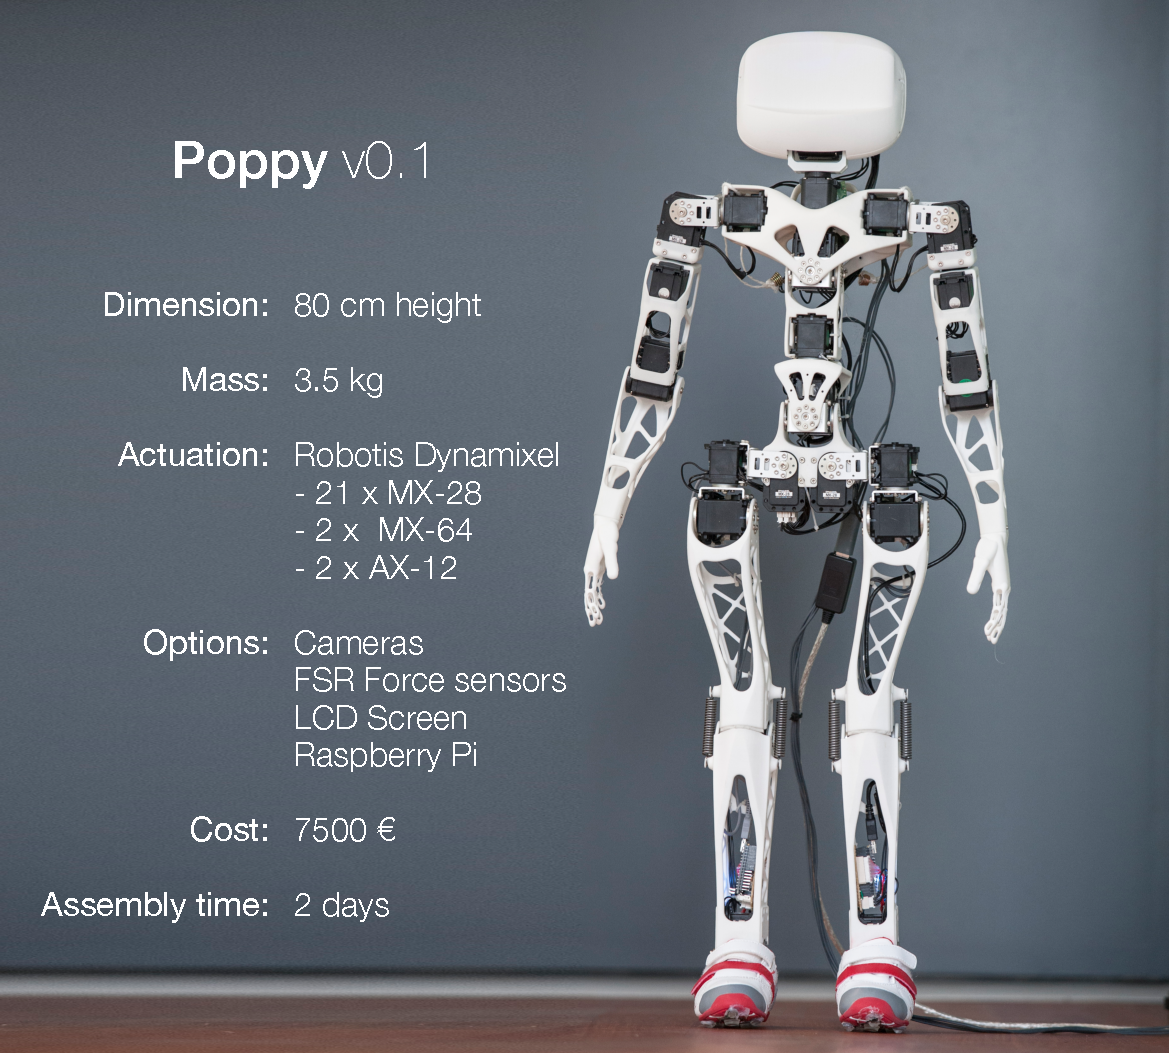
\includegraphics[width=0.95\linewidth]{poppy-overview.pdf}
    \end{center}
    \caption{}
    \label{fig:poppyv0.1_overview}
\end{figure}

Poppy is designed to conduct robotic experiments and integrates several key abilities in an easy-to-use robotic platform toward creating a friendly research framework:
\begin{itemize}
    \item \textbf{Modular morphology}: Poppy is fully modular (mechanic, electronic, software) allowing to freely explore and modify Poppy's body.
    \item \textbf{Social and physical human-robot interaction:} Poppy was designed to afford full-body physical interaction, as well as to afford social interaction, with a head and gestural apparatus that can be programmed for communicative or affective expression.
    \item \textbf{Full-body compliance:} Important aspects of adaptation to physical obstacles or to humans require humanoid robots to be full-body compliant. The use of Robotis Dynamixel actuators permits to actively and dynamically control the compliance of motors, which may be either controlled in position with compliance, or directly in torque
    \item \textbf{A particular design:} Poppy is often complimented for its unique design which draws particular attention.
    \item \textbf{Large sensori-motor space:} Robotis Dynamixel give access to a large number of internal sensors and control parameter. In addition, Poppy has several basic sensors such as IMU, camera and which can be easily extended with novel sensors thanks to the Arduino eletronic architecture.
    \item \textbf{Highly hackable:} Its modularity and the use of 3D printing make Poppy higly hackable. It can be easily adapted to particular experimental setups.
    \item \textbf{Easy to duplicate:} the overall time to assemble all mechanic components of Poppy takes about 2 days. Adding extra sensors is simplified by the use of Arduino electronic architecture.
    \item \textbf{Robustness:} Poppy is designed to be robust to falls and to allow long experimentations (e.g. several hours). Also, its conception, slightly under-actuated, prevents it from destructing itself if wrong moves occur.
    \item \textbf{Transportable outside the lab:} Its size (84 cm) and weight (3.5 kg) make Poppy an easily tranportable robot. In addition its robustness avoid the installation of complex security system around the platform allowing the use Poppy anywhere.
    \item \textbf{Easy to setup:} we try to keep Poppy and its modules as Plug’n'Play as possible.
    \item \textbf{Affordable:} to make Poppy widely accessible, we keep the cost relatively low. You can afford all components for 7500-8000\texteuro or thanks to its modularity, only use the parts of the robot needed.
\end{itemize}


Also we set up several web tools to support collaboration and sharing among members of the Poppy community: a portal web site (\url{www.poppy-project.org}), GitHub repositories for the hardware and software with associated wikis for documentation (\url{www.github.com/poppy-project/}), and a novel generation forum based on Discourse\footnote{\url{www.discourse.org}} technology (\url{forum.poppy-project.org}).



\section{Highlight of some Poppy's morphological aspects}


\subsection{Bio-inspired body} % (fold)
Toward the design and the exploration of an adapted mechanical structure for biped locomotion, we interested ourselves in how evolution solved sensorimotor tasks related to locomotion and in particular bipedal locomotion. As human locomotion represents one of the finest example of mastering bipedal walking, we took functional inspiration of some elements that seem relevant to improve the locomotion of humanoid robots also the morphological optimization is mainly expressed on the locomotive system (legs and trunks) in order to increase the robot robustness, agility and stability during the walking.

\subsubsection{Human proportion} % (fold)
This bio-inspiration is expressed on the whole structure of Poppy. On the anatomical point of view, it reproduces the human proportions as described in the literature~\cite{dufour2005biomecanique}  (see \figurename~\ref{fig:proportion_poppy}) and their sensorimotor space organization: i.e. the main degrees of freedom (actuated and passive), an inertial unit in the head.

\begin{figure}[]
    \centering
    \includegraphics[width=0.9\linewidth]{proportion_poppy.jpg}
    \caption{Human proportion used for the design of Poppy~\cite{dufour2005biomecanique}}
    \label{fig:proportion_poppy}
\end{figure}

\subsubsection{A multi-articulated trunk} % (fold)

Poppy uses the bio-inspired trunk system introduced by Acroban~\cite{ly2010}. Involving five articulations, it allows the reproduction of the main DOFs of the human spine. This feature permits the production of more natural and fluid motions while improving the user experience during physical interaction (see \figurename~\ref{fig:poppy_multi_articulated_trunk}). In addition, the spine plays a fundamental role in bipedal walking and postural balance by actively participating in the balancing of the robot.

\begin{figure}[]
\centering
    \subfloat[][]{\label{fig:frontal_trunk}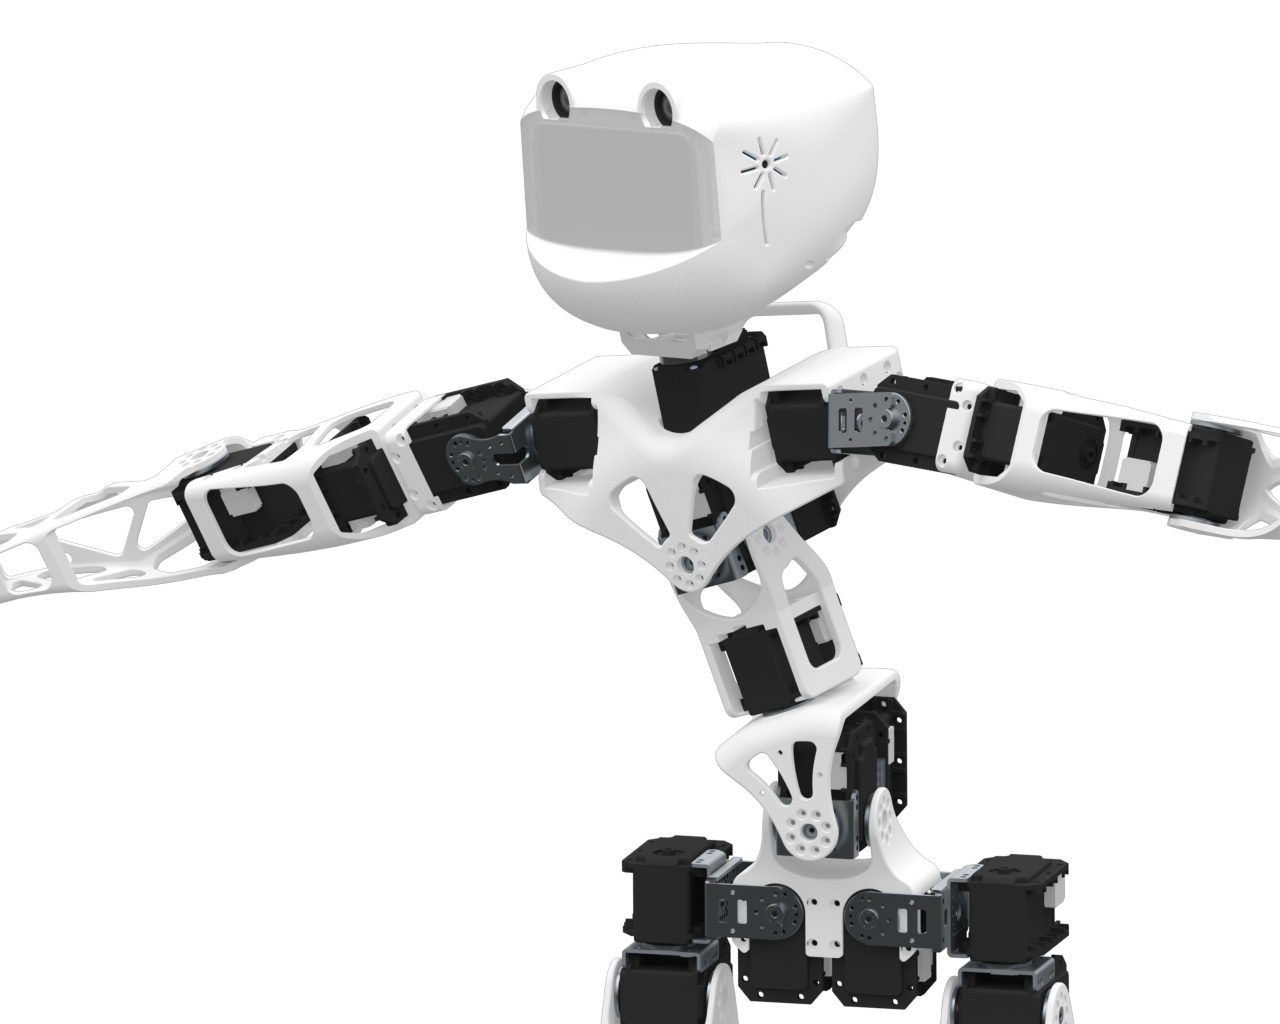
\includegraphics[width=0.49\linewidth]{trunk_face.png}}
    \hfil
    \subfloat[][]{\label{fig:sagittal_trunk}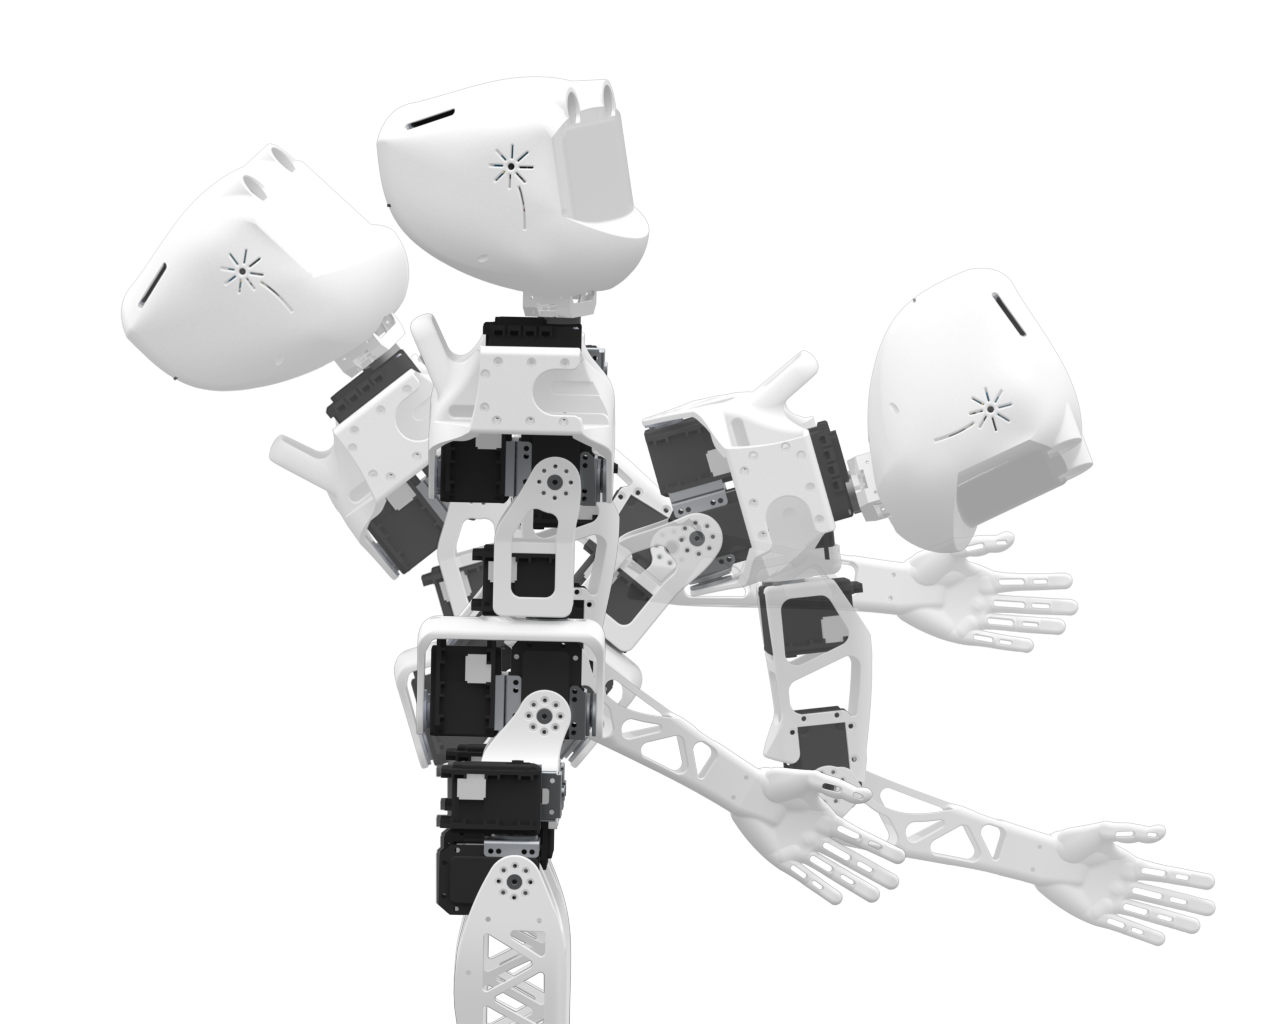
\includegraphics[width=0.49\linewidth]{trunk_sagittal.png}}
    \caption{Poppy has an articulated trunk of 5 DoFs which allows more natural and fluid motions while improving the user experience during physical interaction and actively participating to the balance of the robot.}
    \label{fig:poppy_multi_articulated_trunk}
\end{figure}

% Contrary to the design of the hips, it was not possible here to fit the 5 motors in the frontal plane due to the limited space in the trunk. So to reduce the shifting of the center of gravity to the back of the robot we gradually shifted the upper body to the front. By doing so, we keep the CoG in the support polygon.

\subsubsection{The bio-inspired thigh} % (fold)
The shape of the thigh is inspired of the human thigh. It is bended by angle of 6\textsuperscript{o}, increasing the stability of the robot during biped locomotion. In the chapter~\ref{REF} we will compare this design with a more traditional straight thigh. We will describe both the theoretical model and real experiments showing that the bio-inspired thigh allows the reduction of falling speed by almost 60\% (single support phase) and the decrease of the lateral motion needed for the mass transfer from one foot to the other by 30\% (double support phase) while reducing the upper body perturbation by about 45\% indicating a more stable walk.

\subsubsection{Foot design} % (fold)

To allow efficient and human-like walking gait, Poppy's feet design takes some functional inspiration from the actual human foot such as the proportion, compliance and toes which are key features concerning both the human walking and biped robots with a human-like gait. In addition, we wanted to reduce the weight (i.e. reducing inertia) of the feet to increase the robot agility. To keep the foot as light as possible while conserving functional properties we decided to use a single motor for the main motion (sagittal plane) while other DoF are passives.

The lateral motion of the foot is limited: few range of motion, low torque. The need of a 360 deg and high torque motor seems over rated. Technically the addition of a motor lead to a major weight gain. We preferred to design  instead a passive joint using torsion spring.

\textbf{Author's note:} A new feet is currently under development and will be released in the incoming weeks. This part will be updated.

\subsection{Lightweight and compliant structure} % (fold)
Following ecological principles~\cite{pfeifer2005new} we decided to design a lightweight and compliant robot requiring low actuation power. All our design choices, such as the materials, the motors or the sensors, have been made to have a balanced morphology.

Weight reduction was achieved through the use of trellis structures. These structures, mainly used in civil engineering, are among the best technical solutions to optimize the weight/resistance ratio. All the limbs of Poppy are based on this structure and have been optimized using finite element analysis (FEA) to perform structural simulation and validate parts performance and safety factors.

In the next sections we will detail each part of the robot and how they fit within these designs principles.

% \subsubsection{Actuation} % (fold)
% \label{ssub:robot_actuation}
% However these motors are quite heavy (72, 126 and 153g respectively for MX-28, MX-64 and MX-106) in comparison of the Futaba servo-motors\footnote{\url{http://www.futaba-rc.com/servos/brushless.html}}, 20-50g for a comparable output torque. Given these constraints, the challenge consists in minimizing the number of motors and the power needed to reduce the global weight of the robot.

\subsubsection{Material properties} % (fold)
\label{ssub:material_properties}

All mechanicals parts are made using laser sintering technology. This 3D printing process allows the production of almost any shape without constraint. In addition, the price of the part depends on the total size and not on the complexity of the shape. This permits the production of very optimized shapes without increasing the total price of the robot. Also, this technique is compatible with several materials from polyamide to titanium. Parts manufacturing was subcontracted to an external company\footnote{\url{http://i.materialise.com/}}.
For Poppy's structure we decided to use the polyamide material because it is lightweight and very flexible while keeping good strength properties (see the table~\ref{tab:materials}).

\begin{table}[h]
    \centering
    \begin{tabularx}{0.8\linewidth }{l X X X}
        Material & Mass Density $\rho$ ($kg/m^3$) &  Yield strength $\sigma$~($MPa$) & Young Modulus $E$($GPa$)\\
        \hline
        Polyamide & $930$ & $49$ & $1.65$\\

        Aluminum & $2700$ & $200$ & $70$\\

        Steel & $7500-8000$ & $350$ & $200$\\

        Titanium & $4500$ & $1200$ & $114$\\

    \end{tabularx}

    \caption{Comparison of material properties.
    The Young modulus represents the stiffness of the material while the yield strength corresponds to the maximal stress tolerable before plastic deformation.}
    \label{tab:materials}
\end{table}


\subsubsection{Structure design} % (fold)
\label{ssub:structure_design}

All mechanical parts were designed to optimize their weight and make the platform Poppy as light as possible.
The obtained mass reduction allows the use of less powerful motors which are therefore lighter.
We can thus have a lightweight robot, strong and powerful enough to perform tasks such as walking and physical interaction.

Weight reduction was achieved through the use of trellis structures.
These structures, mainly used in civil engineering, are among the best technical solutions to optimize the weight/resistance ratio.
All the limbs of Poppy are based on this structure and have been optimized using finite element analysis (FEA) to perform structural simulation and validate parts performance and safety factors.


\begin{figure}[!h]
\centering
    \subfloat[][Section of the Poppy's leg]{\label{fig:Poppy_leg_section}\includegraphics[height=4cm]{Poppy_leg_section.jpg}}
    \hfil
    \subfloat[][Equivalent square section]{\label{fig:basic_leg_section}\includegraphics[height=4cm]{basic_leg_section.jpg}}
    \caption{}
    \label{fig:leg_section}
\end{figure}


The main quadratic momentum taken at the middle of the leg given the trellis structure (see \figurename~\ref{fig:leg_section}.a) is:

\begin{center}
    $I_x = \iint_s y^2 dxdy$ and  $I_y = \iint_s x^2 dxdy$

    with $s = dxdy$
\end{center}
\begin{center}
    $I_x = 54.862 mm^4$
    ,
    $I_y = 53.260 mm^4$
\end{center}

For instance, given a solid bar with rectangular profile (\figurename~\ref{fig:leg_section}.b):

{\centering
    $I_x = \frac{b \cdot h^3}{12}$
    ,
    $I_y = \frac{b^3 \cdot h}{12}$
}
It would require a section such as $b=27.72 mm$ and $h=27.59 mm$ to get the same quadratic momentum.
Considering the length of the leg part (i.e.
$190 mm$), the total mass would be equal to $142 g$ instead of $47 g$ for the actual leg.
This corresponds to a reduction of 70\% of the mass.

By using this mesh structure on most of the robot, the total weight of the 3D
printed parts were reduced of about 1.3kg while still being resistant under shocks and falls.


\subsection{Social and emotional skills} % (fold)

In our lab we are especially interested by the role of morphology for dynamic task such as biped locomotion or physical human robot interaction. Yet Poppy is designed to be a multipurpose robot adapted for several kind of scientific exploration.
An important and challenging research topic is the natural human-robot communication so we have provided Poppy with some basic features allowing to directly explore social human-robot interaction and thus extend the potential research community users.

\subsubsection{Expressive head} % (fold)
Strong technical constraints was imposed because the head embed most of electronic components of Poppy plus a wide 4.5" screen and cameras for social communication. Therefore lot of effort have been invested in the design and aesthetic of Poppy's head (see \figurename~\ref{fig:poppy_beta_head}), both its identity and main communication apparatus. It takes inspiration in robotics, animals, object design and art (see the associated pinterest board \url{http://www.pinterest.com/matthieulapeyre/robot/}). We tried to make it cute, expressive and simple.

\begin{figure}[]
\centering
    \subfloat[][The first assembly]{\includegraphics[height=5cm]{head_beta_assembled.jpg}}
    \hfil
    \subfloat[][Screen powered on with basic eyes display]{\includegraphics[height=5cm]{poppy_beta_eyes.jpg}}
    \caption{}
    \label{fig:poppy_beta_head}
\end{figure}

However, in the first version showed here, there is a major design error. Indeed my desire was to have a screen to create and explore freely expressive eyes but the use of two visible cameras changed the way people saw Poppy's head. Of course, people seeing 2 cameras considers they are the eyes of the robot and therefore extrapolate that the screen may be the mouth.

We are working on this issue by replacing the two big camera by a small one with a pinhole lens which can be hidden on the Poppy face.


\subsubsection{Compliant and multi-articulated body} % (fold)

Thanks to its multi-articulated structure and its expressive head, Poppy has a particularly high potential for creating and studying emotions and gesture social communication (see \figurename~\ref{fig:TER_cognitic}).

\begin{figure}[]
\centering
    \subfloat[][\url{http://youtu.be/StFIMuyz11M}]{\includegraphics[width=0.45\linewidth]{TER_surprise.jpg}}
    \hfil
    \subfloat[][\url{http://youtu.be/RwCtNwLk10E}]{\includegraphics[width=0.45\linewidth]{TER_joy.jpg}}\\
    \subfloat[][\url{http://youtu.be/qrcmLXbpUVo}]{\includegraphics[width=0.45\linewidth]{TER_sad.jpg}}
    \hfil
    \subfloat[][\url{http://youtu.be/ms2niFLevv8}]{\includegraphics[width=0.45\linewidth]{TER_fear.jpg}}
    \caption{}
    \label{fig:TER_cognitic}
\end{figure}



\section{The electronical architecture} % (fold)

\section{Pypot: a versatile and modular python control library}

\section{Discussion}

\section{Conclusion}

